\documentclass[aspectratio=169,11pt]{beamer}
\usetheme{Boadilla}
\usecolortheme{seahorse}
\usepackage{booktabs,graphicx}
\setbeamertemplate{navigation symbols}{}
\setbeamertemplate{footline}[frame number]
\title{Checking Semantic Correspondence\\Between English and Lean Proofs}
\author{Taylor Belcher \and ChatGPT (AI collaborator)}
\institute{CSCE883: Machine Learning}
\date{November 2026}
\begin{document}
\begin{frame}\titlepage\end{frame}
\begin{frame}{What are we checking?}
\begin{itemize}
\item Does the Lean proof faithfully represent the supplied English argument?
\item Compare assumptions, conclusions, witnesses, dependencies, and essential steps.
\item Two valid proofs of the same theorem can use different arguments.
\end{itemize}
\begin{block}{A different trust boundary}A correct kernel can verify a formal proof that does not say what the accompanying English says.\end{block}
\end{frame}
\begin{frame}{Why this is a real problem}
\begin{itemize}
\item Navier--Stokes \emph{Lost in Translation}: discrepancies between a manuscript and its cited formalization.
\item FaithformBench: formalizers can silently repair invalid input reasoning.
\item Buzzard's Xena discussion: readable informalization can help inspect formal artifacts.
\item Pollack: checking a derivation and believing the intended claim are distinct tasks.
\end{itemize}
\small Full references and source links are in the paper bibliography. Kernel soundness bugs require a separate kind of check.
\end{frame}
\begin{frame}{The hardest part was the data}
\begin{itemize}
\item ProofNet-Verified corrects statements; proof-route fidelity was an assumption in our experiments.
\item Herald provides paired English and Lean proofs for translation supervision, without our needed human fidelity labels.
\item Swaps produce negatives, but may expose topic or statement shortcuts.
\item Faithform offers relevant perturbed reasoning, with a different annotation unit and scope.
\end{itemize}
\begin{block}{Needed}Human-reviewed faithful and unfaithful argument pairs, with explanations of the differences.\end{block}
\end{frame}
\begin{frame}{Earlier experiments: strong scores, narrow conclusions}
\small\centering
\begin{tabular}{lrr}
\toprule Protocol & Original & Tuned / trained\\\midrule
8B statements (112 validation) & 62.5\% & 70.5\%\\
14B random swaps (118 validation) & 81.4\% & 100.0\%\\
14B related swaps (54 test) & 77.8\% & 98.1\%\\
Paired forest, random swaps (118) & --- & 89.0\%\\\bottomrule
\end{tabular}
\vspace{.4cm}
\begin{itemize}\item Comparisons are within rows; protocols are not interchangeable.
\item 8B tuning increased accuracy while decreasing mismatch recall.
\item An English-only forest reached 91.5\%: evidence of a possible shortcut, not paired checking.\end{itemize}
\end{frame}
\begin{frame}{Holding the theorem fixed exposes a weakness}
For each of four theorems: two English routes $E_A,E_B$ and two Lean routes $L_A,L_B$.
\begin{center}\begin{tabular}{c|cc} & $L_A$ & $L_B$\\\hline $E_A$ & Match & Mismatch\\ $E_B$ & Mismatch & Match\end{tabular}\end{center}
\begin{itemize}\item Example: explicit witness $x=1$ versus the intermediate value theorem for $x^3+x=2$.
\item Original 14B: 15/16; random-swap tuned: 8/16; related-swap tuned: 11/16.
\item Four synthetic families, not 16 independent problems; agent labels, repeated inspection.
\item Ranking and fixed-threshold accuracy can disagree.\end{itemize}
\end{frame}
\begin{frame}{Our main approach: informalize, then compare}
\centering
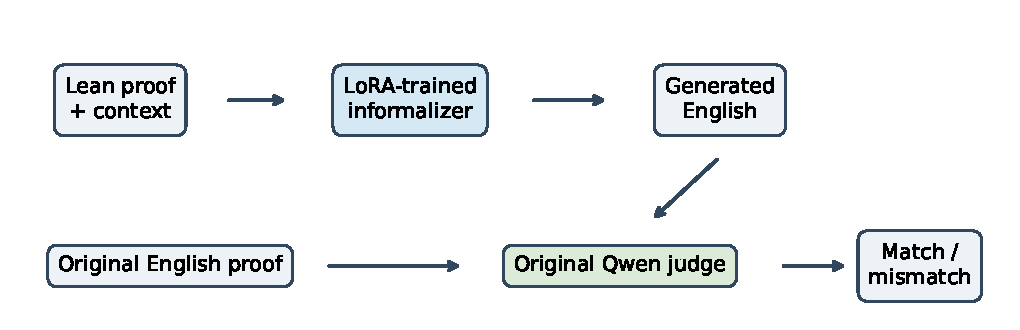
\includegraphics[width=.92\textwidth]{../paper/figures/pipeline.pdf}
\begin{itemize}\item Train only the Lean-to-English translator.
\item Original English is withheld from translation and supplied to the judge.
\item Inspect the generated account to distinguish translation failures from judgment failures.\end{itemize}
\end{frame}
\begin{frame}{Training and evaluation setup}
\begin{itemize}
\item Qwen3-14B, BF16; LoRA rank 16, alpha 32, dropout 0.05; q/k/v/o projections.
\item One epoch; learning rate $10^{-4}$; accumulation 8; seed 883.
\item English completion loss only; 2,048 training tokens, 1,024 target/generation limit; no training truncation.
\item Herald: 4,096 train / 64 validation / 64 test; grouped splitting.
\item Fresh ProofNet run: 176 train / 36 validation; evaluate on 54 related-swap pairs.
\item RTX A6000 (48 GB), 128 GB RAM. Original 14B judge in both runs.
\end{itemize}
\end{frame}
\begin{frame}{Herald: completed translations, not measured accuracy}
\centering
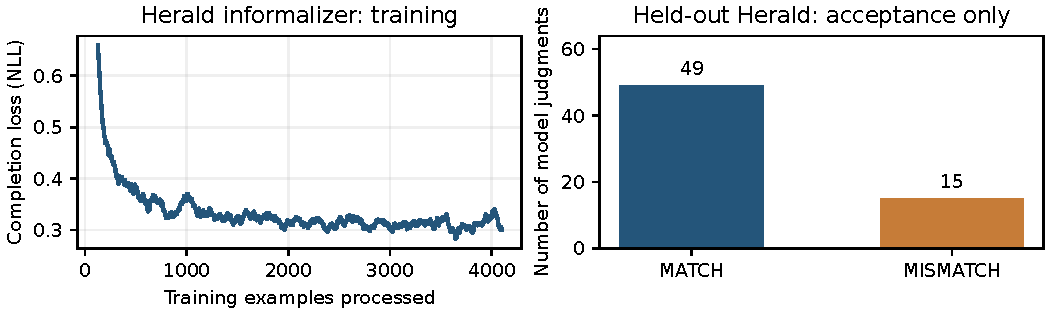
\includegraphics[width=.88\textwidth,height=.56\textheight,keepaspectratio]{../paper/figures/informalization-herald.pdf}
\begin{itemize}\item 64/64 completed: 49 accepted, 15 rejected (76.6\% acceptance).
\item No independent correspondence labels: acceptance is not accuracy.
\item Readable output can still omit an important assumption or helper argument.\end{itemize}
\end{frame}
\begin{frame}{ProofNet: detecting mismatches, rejecting too many matches}
\begin{columns}
\column{.49\textwidth}\small
54 attempted; 46 scored; 8 generation-limit abstentions.
\begin{center}\begin{tabular}{lrr}\toprule Actual / predicted & Mismatch & Match\\\midrule Mismatch & 23 & 0\\ Match & 17 & 6\\\bottomrule\end{tabular}\end{center}
Accuracy 63.0\%; mismatch P/R/F1: .575 / 1.000 / .730.
\medskip
Synthetic/assumed labels; conditional on completion. Strong ranking does not fix false rejections.
\column{.49\textwidth}
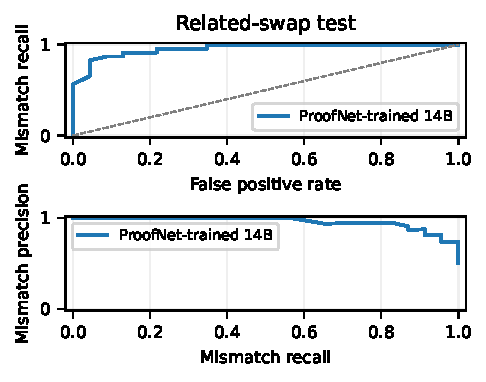
\includegraphics[width=\textwidth]{../paper/figures/informalization-proofnet-curves.pdf}
\end{columns}
\end{frame}
\begin{frame}{OpenAI cases: a flag is not a diagnosis}
\begin{itemize}
\item Two targeted Navier--Stokes cases: inverse estimate and pressure estimate.
\item Herald pipeline flagged both, but its accounts omitted essential assumptions or helper reasoning.
\item ProofNet pipeline: inverse account only 27 tokens; pressure output repeated until the 2,048-token cap (abstention).
\item Neither run reliably identified the documented mathematical discrepancy.
\end{itemize}
\begin{block}{Interpretation}Evaluate the generated explanation and its dependencies, not just whether the final answer says ``mismatch.''\end{block}
\end{frame}
\begin{frame}{Could controlled intermediaries help?}
\begin{itemize}
\item Earlier original-model runs used Lean, English, Verbose Lean, and Natural Lean intermediaries.
\item English, Verbose Lean, and Natural Lean each scored 16/16 on the small same-theorem diagnostic.
\item Related-swap coverage differed substantially; no clean superiority comparison.
\item No complete generated-code comparison pair passed all compiler checks.
\end{itemize}
\begin{block}{Still worth investigating}Structured dependencies and aligned steps may make omissions visible, but intermediary translation adds another possible failure.\end{block}
\end{frame}
\begin{frame}{Limits and next steps}
\begin{itemize}
\item Small open-weight models and token budgets limit long dependency chains.
\item Repeated diagnostics, assumed positives, and synthetic negatives limit generalization claims.
\item Build human-reviewed semantic pairs: both labels, multiple routes, explicit discrepancy evidence.
\item Informalize helper lemmas and track assumptions through the dependency graph.
\item Calibrate on a separate validation set; evaluate translator and judge separately.
\end{itemize}
\small Broader impact: accessible proof explanations could assist review; unsupported automated confidence could mislead it.
\end{frame}
\begin{frame}{Takeaway}
\begin{block}{The main result}High performance on constructed swaps did not establish reliable argument-fidelity checking. Informalization exposes useful evidence, but translation omissions remain a bottleneck.\end{block}
\begin{itemize}\item Preserve the distinction between validity, correspondence, and readability.
\item Better public labels and human review are essential to measure progress.
\end{itemize}
\small Code, evidence, report, and supplement:\\
\url{https://github.com/hotdogontology/CSCE883/tree/main/Homework/Project}
\end{frame}
\end{document}
